% Asal-usul (tidak pernah dicetak): lihat sources/outline_sources.md (Tahun 1: tegangan dan
% tegangan utama dalam 2D; regangan; geser murni dan sederhana; perilaku elastik, rapuh dan
% duktil; amplop kekuatan litosfer). Amplop kekuatan dari figdata/bachelor-1/strength_envelope.py
% (Byerlee 1975; hukum aliran Gleason dan Tullis 1995 serta Hirth dan Kohlstedt 2003 sebagaimana
% disusun oleh Lopez-Sanchez; geoterm bab 10); nilai soal latihan dan soal dihitung dalam kalkulator
% skrap Buku 3 calc/ch16.py. Traksi, tegangan geser, tensor tegangan dan regangan, hukum Hooke,
% modulus Young dan viskositas termasuk dalam seri fisika dan diingat kembali, tidak didefinisikan
% ulang (ketetapan sinkronisasi 1).
\chapter{Tegangan, regangan dan reologi}\label{ch:b1:stress-strain-rheology}

Pada 1960-an, air limbah yang dipompa ke sumur pembuangan di Rocky Mountain Arsenal, dekat Denver, menyebar ke dalam batuan dasar kristalin yang retak antara \qty{3.7}{km} dan \qty{7.0}{km} di bawah permukaan, dan gempa bumi menyusul. Gempa-gempa itu tetap berada di dalam bagian batuan tempat tekanan fluida telah naik lebih dari sekitar \qty{3.2}{MPa}.
% ledger: hb81:denver
Setengah abad kemudian hal yang sama terjadi dalam skala yang lebih besar di Oklahoma, tempat air asin yang terbawa bersama minyak dan gas dipompa kembali ke bawah tanah. Di dalam dan sekitar negara bagian itu, gempa bumi bermagnitudo 3 atau lebih berjumlah satu hingga lima per tahun dari 2005 hingga 2008, lalu \num{20} pada 2009, \num{585} pada 2014 dan \num{888} pada 2015, lebih dari dua per hari; guncangan bermagnitudo 5.7 dan 5.8 mengguncang Prague, pada 2011, dan Pawnee, pada 2016. Empat sumur pembuangan bervolume tinggi saja dapat menjelaskan seperlima gempa bumi di Amerika Serikat tengah, dan memicu sebagian yang berjarak lebih dari \qty{30}{km}.
% ledger: usgs:oklahoma-rate, usgs:prague-pawnee, keranen:oklahoma
Air itu tidak mendorong apa pun ke samping; ia hanya menaikkan tekanan fluida di dalam pori-pori batuan. Mengapa itu membuat sebuah sesar tergelincir? Jawabannya memerlukan tiga gagasan, yang menjadi pokok bab ini: tegangan pada bidang di dalam batuan, kondisi tempat bidang itu menyerah, dan fakta bahwa \omterm{def:b1:stress-strain-rheology:lithostatic}{tekanan fluida pori} bekerja melawan gaya yang menekan kedua sisi bersama. Dengan ketiganya, dan dengan hukum rayapan untuk batuan panas, kita dapat menggambar kekuatan seluruh \omterm{def:b1:layered-earth:lithosphere}{litosfer} terhadap kedalaman.

\begin{recall}
Gaya yang tersebar pada suatu permukaan bekerja melalui gaya per satuan luasnya, dalam pascal; tekanan dalam fluida diam bertambah dengan kedalaman sebagai $\rho g z$ (buku fisika). Pegas, dan padatan dalam deformasi kecil, mematuhi hukum Hooke: regangan sebanding dengan tegangan, dengan modulus Young sebagai konstanta; fluida kental menahan sebanding dengan laju gesernya, dengan viskositas sebagai konstanta. Buku fisika volume Tahun ke-3 menggambarkan tegangan dan regangan dalam tiga dimensi dengan tensor; bab ini hanya memerlukan dua. Matriks $2\times2$ simetris memiliki dua nilai eigen real dan dua vektor eigen yang tegak lurus (matematika, Tahun 1). \omterm{def:b1:heat-budget:geotherm}{Geoterm} pada \cref{ch:b1:heat-budget} memberi suhu pada kedalaman; sesar telah ditemui di Buku 1, kelas 7.
\end{recall}

\section{Tegangan dalam dua dimensi}\label{sec:b1:stress-strain-rheology:stress}

Potong sebuah batuan dalam pikiran sepanjang permukaan datar kecil. Batuan di satu sisi menekan batuan di sisi lain dengan gaya, dan gaya per satuan luas adalah traksi pada permukaan itu, dalam istilah buku fisika. Arahnya, pada umumnya, bukan arah normal terhadap permukaan.

\begin{definition}[Tegangan normal]\label{def:b1:stress-strain-rheology:stress}
Pada suatu bidang melalui sebuah titik batuan, gaya per satuan luas yang dikerjakan batuan di satu sisi pada sisi lain memiliki komponen sepanjang normal bidang, \emph{tegangan normal}\index{tegangan normal} $\sigma_n$, dan komponen sepanjang bidang, tegangan geser $\tau$. Dalam ilmu kebumian tegangan normal dihitung positif ketika ia memampatkan.
\end{definition}

Konvensi tandanya berlawanan dengan konvensi insinyur. Ia dipilih karena hampir setiap tegangan di Bumi padat adalah kompresi: berat batuan di atas menekan segala sesuatu di bawahnya.

Kita bekerja pada bidang vertikal, dengan sumbu $x$ horizontal dan sumbu $y$. Pada bidang yang tegak lurus $x$ \omterm{def:b1:stress-strain-rheology:stress}{tegangan normalnya} adalah $\sigma_{xx}$ dan tegangan gesernya $\sigma_{xy}$; pada bidang yang tegak lurus $y$ keduanya adalah $\sigma_{yy}$ dan $\sigma_{yx}$. Kedua tegangan geser itu sama: pada sebuah kotak kecil, gaya geser pada sisi-sisi vertikal membentuk kopel dengan momen $\sigma_{xy}a\cdot a$ untuk sisi $a$, dan yang pada sisi-sisi horizontal kopel $\sigma_{yx}a\cdot a$ yang berputar ke arah sebaliknya, dan kotak itu akan berputar jika keduanya berbeda. Jadi tiga bilangan menggambarkan tegangan pada sebuah titik, dan itu cukup untuk memberikannya pada setiap bidang.

\begin{proposition}[Tegangan pada bidang miring]\label{prop:b1:stress-strain-rheology:transformation}
Misalkan sebuah bidang memiliki normal satuan $\vec n = (\cos\theta, \sin\theta)$, pada sudut $\theta$ dari sumbu $x$, dan misalkan $\vec m = (-\sin\theta, \cos\theta)$ menjadi vektor satuan sepanjang bidang itu. \omterm{def:b1:stress-strain-rheology:stress}{Tegangan normal} dan geser pada bidang itu
adalah vektor satuan sepanjang bidang itu. \omterm{def:b1:stress-strain-rheology:stress}{Tegangan normal} dan geser pada bidang itu adalah
\begin{align*}
  \sigma_n &= \sigma_{xx}\cos^2\theta + 2\sigma_{xy}\sin\theta\cos\theta + \sigma_{yy}\sin^2\theta
           = \frac{\sigma_{xx}+\sigma_{yy}}{2} + \frac{\sigma_{xx}-\sigma_{yy}}{2}\cos2\theta + \sigma_{xy}\sin2\theta, \\
  \tau     &= (\sigma_{yy}-\sigma_{xx})\sin\theta\cos\theta + \sigma_{xy}(\cos^2\theta - \sin^2\theta)
           = -\frac{\sigma_{xx}-\sigma_{yy}}{2}\sin2\theta + \sigma_{xy}\cos2\theta ,
\end{align*}
dengan $\tau$ dihitung positif sepanjang $\vec m$.
\end{proposition}

\begin{proof}
Potong sebuah prisma kecil, seperti pada gambar di bawah: sebuah bidang miring dengan luas $A$ dan normal keluar $\vec n$, sebuah bidang vertikal dengan luas $A\cos\theta$ dan sebuah bidang horizontal dengan luas $A\sin\theta$, per satuan panjang pada arah ketiga. Berat dan inersianya sebanding dengan volumenya, yang menyusut lebih cepat daripada bidang-bidangnya; untuk prisma yang cukup kecil, gaya pada bidang-bidangnya harus seimbang dengan sendirinya. Karena kompresi dihitung positif, batuan di luar mendorong bidang vertikal dengan gaya $A\cos\theta\,(\sigma_{xx}, \sigma_{xy})$ dan bidang horizontal dengan $A\sin\theta\,(\sigma_{xy}, \sigma_{yy})$; pada bidang miring ia mendorong dengan $-A(\sigma_n\vec n + \tau\vec m)$. Jumlahnya nol:
\[
  \sigma_n\vec n + \tau\vec m = \cos\theta\,(\sigma_{xx}, \sigma_{xy}) + \sin\theta\,(\sigma_{xy}, \sigma_{yy}) .
\]
Hasil kali skalar dengan $\vec n$ memberi $\sigma_n$, dengan $\vec m$ memberi $\tau$, karena $\vec n\cdot\vec m = 0$. Bentuk kedua mengikuti dari $\cos^2\theta = (1+\cos2\theta)/2$, $\sin^2\theta = (1-\cos2\theta)/2$ dan $2\sin\theta\cos\theta = \sin2\theta$.
\end{proof}

\begin{omfigure}
\begin{tikzpicture}[>={Stealth[length=5pt]}, font=\small]
% theta = 35 deg, hypotenuse L = 4.5: a = L cos(theta), b = L sin(theta)
\pgfmathsetmacro{\th}{35}
\pgfmathsetmacro{\L}{4.5}
\pgfmathsetmacro{\a}{\L*cos(\th)}
\pgfmathsetmacro{\b}{\L*sin(\th)}
\coordinate (O) at (0,0);
\coordinate (A) at (0,\a);
\coordinate (B) at (\b,0);
\coordinate (M) at ($(A)!0.5!(B)$);
\fill[omLithGranite!45] (O) -- (A) -- (B) -- cycle;
\draw[line width=0.8pt] (O) -- (A) -- (B) -- cycle;
% axes
\draw[->, black!70] (-2.6,-1.9) -- (-1.6,-1.9) node[right] {$x$};
\draw[->, black!70] (-2.6,-1.9) -- (-2.6,-0.9) node[above] {$y$};
% face on x = 0 (outward normal -x), area A cos(theta)
\draw[->, line width=1.1pt, omDef] (-1.35,0.5*\a) -- (-0.05,0.5*\a);
\node[omDef, anchor=south] at (-0.95,0.5*\a+0.05) {$\sigma_{xx} A\cos\theta$};
\draw[->, line width=1.1pt, omProp] (-0.25,0.5*\a-1.25) -- (-0.25,0.5*\a-0.25);
\node[omProp, anchor=east] at (-0.3,0.5*\a-0.85) {$\sigma_{xy} A\cos\theta$};
% face on y = 0 (outward normal -y), area A sin(theta)
\draw[->, line width=1.1pt, omDef] (0.68*\b,-1.35) -- (0.68*\b,-0.05);
\node[omDef, anchor=west] at (0.68*\b+0.05,-1.05) {$\sigma_{yy} A\sin\theta$};
\draw[->, line width=1.1pt, omProp] (0.1,-0.25) -- (1.1,-0.25);
\node[omProp, anchor=north east] at (0.9,-0.32) {$\sigma_{xy} A\sin\theta$};
% inclined face, area A, normal n = (cos theta, sin theta)
\draw[->, line width=1.1pt, omThm] ($(M)+(\th:1.5)$) -- ($(M)+(\th:0.05)$);
\node[omThm, anchor=south west, inner sep=1pt] at ($(M)+(\th:1.5)$) {$\sigma_n A$};
\draw[->, line width=1.1pt, omThm!70!black] ($(M)+(\th:0.25)+(\th-90:0.75)$) -- ($(M)+(\th:0.25)+(\th-90:1.75)$);
\node[omThm!70!black, anchor=west] at ($(M)+(\th:0.3)+(\th-90:1.3)$) {$\tau A$};
\draw[->, black!70, dashed] ($(M)+(\th+90:1.25)$) -- ++(\th:1.0) node[pos=1, anchor=south west, inner sep=1pt, text=black] {$\boldsymbol n$};
% angle theta at A, between the face and the y axis
\pic[draw, angle radius=0.75cm, pic text={$\theta$}, angle eccentricity=1.35] {angle = O--A--B};
\end{tikzpicture}
\par\smallskip{\small Keseimbangan gaya pada sebuah prisma segitiga kecil batuan. Bidang miring memiliki luas $A$ dan normal satuan $\vec n$; bidang vertikal dan horizontal memiliki luas $A\cos\theta$ dan $A\sin\theta$. Biru: gaya normal pada kedua bidang kecil; oranye: gaya geser pada keduanya; merah: gaya normal dan geser pada bidang miring. Kompresi dihitung positif, sehingga setiap gaya normal menunjuk ke dalam prisma.}
\label{fig:b1:stress-strain-rheology:prism}
\end{omfigure}

\begin{theorem}[Tegangan utama]\label{thm:b1:stress-strain-rheology:principal}
Pada setiap titik batuan terdapat dua bidang yang saling tegak lurus tempat tegangan gesernya nol. \omterm{def:b1:stress-strain-rheology:stress}{Tegangan normal} pada keduanya adalah \omterm{def:b1:stress-strain-rheology:stress}{tegangan normal} terbesar dan terkecil di atas semua bidang melalui titik itu,
\[
  \sigma_{1,3} = \frac{\sigma_{xx}+\sigma_{yy}}{2} \pm
  \sqrt{\Bigl(\frac{\sigma_{xx}-\sigma_{yy}}{2}\Bigr)^2 + \sigma_{xy}^2},
  \qquad \tan2\theta_p = \frac{2\sigma_{xy}}{\sigma_{xx}-\sigma_{yy}},
\]
dengan $\theta_p$ adalah sudut dari sumbu $x$ ke normal bidang yang membawa $\sigma_1$.
\end{theorem}

\begin{proof}
Tulis $c = (\sigma_{xx}+\sigma_{yy})/2$, dan pilih $R \ge 0$ dan $\theta_p$
dengan $(\sigma_{xx}-\sigma_{yy})/2 = R\cos2\theta_p$ dan
$\sigma_{xy} = R\sin2\theta_p$; maka
$R = \sqrt{((\sigma_{xx}-\sigma_{yy})/2)^2 + \sigma_{xy}^2}$ dan
$\tan2\theta_p$ seperti yang dinyatakan. Bentuk kedua dari
\cref{prop:b1:stress-strain-rheology:transformation} menjadi
\[
  \sigma_n = c + R\cos(2\theta - 2\theta_p), \qquad \tau = -R\sin(2\theta - 2\theta_p).
\]
\omterm{def:b1:stress-strain-rheology:stress}{Tegangan normal} terbesar, $c + R$, untuk $\theta = \theta_p$, dan terkecil,
$c - R$, untuk $\theta = \theta_p + \ang{90}$; pada keduanya $\tau = 0$. Perhatikan juga
bahwa $\mathrm d\sigma_n/\mathrm d\theta = 2\tau$: \omterm{def:b1:stress-strain-rheology:stress}{tegangan normal} stasioner tepat di tempat
tegangan geser lenyap.
\end{proof}

\begin{definition}[Tegangan utama, tegangan diferensial]\label{def:b1:stress-strain-rheology:principal}
\emph{Tegangan utama}\index{tegangan utama} pada sebuah titik adalah \omterm{def:b1:stress-strain-rheology:stress}{tegangan normal}
$\sigma_1 \ge \sigma_3$ pada kedua bidang yang bebas dari tegangan geser, dan arahnya adalah
arah utama. Dalam tiga dimensi terdapat tiga, $\sigma_1 \ge \sigma_2 \ge \sigma_3$, pada tiga
bidang yang saling tegak lurus. \emph{Tegangan diferensial}\index{tegangan diferensial} adalah $\sigma_1 - \sigma_3$, dan tegangan rata-rata dalam bidang adalah
$(\sigma_1+\sigma_3)/2$.
\end{definition}

Keadaan tegangan paling mudah dibaca pada arah utamanya. Jika kita mengukur sudut $\theta$
dari arah $\sigma_1$, alih-alih dari sumbu $x$, rumusnya kehilangan suku terakhirnya.

\begin{proposition}[Lingkaran Mohr]\label{prop:b1:stress-strain-rheology:mohr}
Pada bidang yang normalnya membentuk sudut $\theta$ dengan arah $\sigma_1$,
\[
  \sigma_n = \frac{\sigma_1+\sigma_3}{2} + \frac{\sigma_1-\sigma_3}{2}\cos2\theta,
  \qquad
  |\tau| = \frac{\sigma_1-\sigma_3}{2}\,|\sin2\theta| .
\]
Ketika $\theta$ berputar, titik $(\sigma_n, |\tau|)$ menelusuri setengah atas lingkaran dengan pusat $((\sigma_1+\sigma_3)/2,\, 0)$ dan jari-jari $(\sigma_1-\sigma_3)/2$, pada sudut $2\theta$ dari ujung $\sigma_1$-nya. Tegangan geser terbesar, $(\sigma_1-\sigma_3)/2$, bekerja pada bidang-bidang yang membentuk \ang{45} dengan arah utama.
\end{proposition}

\begin{proof}
Dalam sumbu utama $\sigma_{xx} = \sigma_1$, $\sigma_{yy} = \sigma_3$ dan
$\sigma_{xy} = 0$, dan \cref{prop:b1:stress-strain-rheology:transformation}
memberikan kedua rumus itu. Maka
$(\sigma_n - (\sigma_1+\sigma_3)/2)^2 + \tau^2 = ((\sigma_1-\sigma_3)/2)^2$, persamaan
lingkaran itu; $|\sin2\theta|$ terbesar untuk $\theta = \ang{45}$.
\end{proof}

Tanda $\tau$ hanya menyatakan ke arah mana kedua sisi akan meluncur, sehingga setengah atas lingkaran biasanya digambar sendiri. Konstruksi ini dinamai menurut insinyur Christian Otto Mohr, yang juga membangun di atasnya sebuah kriteria keruntuhan, dan ke sanalah kita menuju (\cref{sec:b1:stress-strain-rheology:rheology}).

\subsection*{Tegangan pada kedalaman}

\begin{definition}[Tekanan litostatik, tekanan fluida pori, tegangan efektif]\label{def:b1:stress-strain-rheology:lithostatic}
Pada kedalaman $z$, berat batuan di atasnya, per satuan luas horizontal, adalah tegangan vertikal $\sigma_v = \int_0^z\rho g\,\mathrm dz'$, yang sama dengan $\rho g z$ dalam lapisan dengan massa jenis seragam $\rho$. Ketika tegangan sama di setiap arah dan sama dengannya, batuan berada di bawah \emph{tekanan
litostatik}\index{tekanan litostatik}. Tekanan air, minyak atau gas di dalam pori dan retakan batuan adalah \emph{tekanan fluida
pori}\index{tekanan fluida pori} $P$; ia hidrostatik, $P = \rho_w g z$, ketika pori-pori terhubung ke permukaan. \emph{Tegangan efektif}\index{tegangan efektif} adalah tegangan dikurangi tekanan pori, $\sigma' = \sigma - P$, pada setiap bidang; $\lambda = P/\sigma_v$ adalah rasio tekanan pori.
\end{definition}

Dalam \omterm{def:b1:layered-earth:layers}{kerak} dengan massa jenis \qty{2700}{kg.m^{-3}}, tegangan vertikal bertambah sekitar $2700\times9.81\times1000 = \qty{26.5}{MPa}$ per kilometer dan tekanan pori hidrostatik sebesar \qty{9.81}{MPa} per kilometer: $\lambda = 1000/2700 = 0.37$. Fluida pori mendorong butiran-butiran terpisah dengan tekanan yang sama di setiap arah; ia tidak mengambil apa pun dari tegangan geser, tetapi ia mengambil $P$ dari setiap \omterm{def:b1:stress-strain-rheology:stress}{tegangan normal}. Di tempat pori-pori tersegel, misalnya oleh lempung atau garam, fluida dapat menanggung sebagian berat batuan di atasnya, dan $\lambda$ naik menuju 1.

Tegangan dalam \omterm{def:b1:layered-earth:layers}{kerak} tidak litostatik. Lempeng-lempeng mendorong dan menarik, \omterm{def:b1:layered-earth:layers}{kerak} membengkok, pegunungan menekan akarnya, dan tegangan horizontal berbeda dari yang vertikal. Dekat permukaan, yang tidak menanggung tegangan geser, salah satu arah utama vertikal, seperti ditunjukkan \cref{ch:b1:faults-folds-fabrics}: $\sigma_v$ adalah $\sigma_1$, $\sigma_2$ atau $\sigma_3$, dan ketiga kasus itu adalah tiga cara sesar bergerak.

\section{Regangan}\label{sec:b1:stress-strain-rheology:strain}

Tegangan adalah sebab; regangan adalah yang direkam batuan. Fosil yang ditarik memanjang, kerikil yang dipipihkan, lapisan yang dipendekkan menjadi \omterm{def:b1:geological-maps:fold}{lipatan} semuanya mengukur perubahan bentuk.

\begin{definition}[Perpanjangan, peregangan, regangan geser]\label{def:b1:stress-strain-rheology:strain}
Sebuah garis bahan dengan panjang $\ell_0$ yang terdeformasi menjadi panjang $\ell$ memiliki \emph{perpanjangan}\index{perpanjangan (regangan)} $e = (\ell - \ell_0)/\ell_0$ dan \emph{peregangan}\index{peregangan} $S = \ell/\ell_0 = 1 + e$; pemendekan adalah perpanjangan negatif, peregangan di bawah 1. Dua garis bahan yang tadinya tegak lurus dan kini membentuk sudut $\ang{90} - \psi$ telah tergeser sebesar sudut $\psi$, dan \emph{regangan geser}\index{regangan geser} adalah $\gamma = \tan\psi$.
\end{definition}

Regangan homogen ketika setiap daerah kecil batuan terdeformasi dengan cara yang sama. Posisi baru $\vec x'$ dari titik $\vec x$ kemudian merupakan fungsi linear, $\vec x' = F\vec x$, dengan matriks konstan $2\times2$ $F$ (dan $\det F > 0$, karena batuan tidak terbalik ke dalam). Garis lurus tetap lurus dan garis sejajar tetap sejajar; persegi menjadi jajar genjang, dan lingkaran menjadi elips.

\begin{proposition}[Elips regangan]\label{prop:b1:stress-strain-rheology:ellipse}
Di bawah regangan homogen $\vec x' = F\vec x$, lingkaran berjari-jari 1 menjadi elips yang semi-sumbunya adalah akar kuadrat $S_1 \ge S_2$ dari nilai eigen $FF^{\mathsf T}$, sepanjang vektor eigennya yang tegak lurus. $S_1$ dan $S_2$ adalah \omterm{def:b1:stress-strain-rheology:strain}{peregangan} terbesar dan terkecil dari semua garis bahan, dan luasnya dikalikan $\det F = S_1S_2$.
\end{proposition}

\begin{proof}
Titik $\vec x = F\vec u$ berasal dari sebuah titik $\vec u$ pada lingkaran, $|\vec u| = 1$, sehingga $|F^{-1}\vec x|^2 = 1$, yaitu $\vec x^{\mathsf T}(FF^{\mathsf T})^{-1}\vec x = 1$. Matriks $B = FF^{\mathsf T}$ simetris dengan nilai eigen positif $\lambda_1 \ge
\lambda_2$ ($\vec v^{\mathsf T}B\vec v = |F^{\mathsf T}\vec v|^2 > 0$); dalam vektor eigennya yang tegak lurus, persamaannya menjadi
$x_1^2/\lambda_1 + x_2^2/\lambda_2 = 1$, sebuah elips dengan semi-sumbu $\sqrt{\lambda_1}$ dan $\sqrt{\lambda_2}$. Sebuah garis bahan sepanjang vektor satuan $\vec u$ memiliki \omterm{def:b1:stress-strain-rheology:strain}{peregangan} $|F\vec u|$, dan
$|F\vec u|^2 = \vec u^{\mathsf T}F^{\mathsf T}F\vec u$ berada di antara nilai eigen $F^{\mathsf T}F$, yang sama dengan nilai eigen $FF^{\mathsf T}$. Akhirnya
$\lambda_1\lambda_2 = \det B = (\det F)^2$.
\end{proof}

\begin{definition}[Elips regangan]\label{def:b1:stress-strain-rheology:strain-ellipse}
\emph{Elips regangan}\index{elips regangan} adalah elips tempat regangan homogen memutar lingkaran berjari-jari 1; semi-sumbunya adalah \omterm{def:b1:stress-strain-rheology:strain}{peregangan} utama $S_1 \ge S_2$, dan sumbunya adalah arah utama regangan.
\end{definition}

Dua regangan yang mengubah bentuk suatu benda secara sama dapat sangat berbeda.

\begin{definition}[Geser murni, geser sederhana]\label{def:b1:stress-strain-rheology:shear-types}
Sebuah \emph{geser murni}\index{geser murni} adalah regangan homogen yang mempertahankan luas dan
mempertahankan arah utamanya tetap dalam batuan:
$F = \begin{pmatrix} k & 0 \\ 0 & 1/k\end{pmatrix}$ dalam sumbu-sumbu itu, dengan
$k > 1$. Sebuah \emph{geser sederhana}\index{geser sederhana} menggerakkan setiap titik sejajar dengan
satu arah, arah geser, sebesar $\gamma$ kali jaraknya dari bidang tetap yang sejajar dengannya:
$F = \begin{pmatrix} 1 & \gamma \\ 0 & 1\end{pmatrix}$.
\end{definition}

Keduanya mempertahankan luas, karena kedua determinannya 1. Pada \omterm{def:b1:stress-strain-rheology:shear-types}{geser murni} garis-garis bahan di sepanjang sumbu \omterm{def:b1:stress-strain-rheology:strain-ellipse}{elips regangan} adalah garis yang sama pada setiap tahap: regangannya koaksial. Pada \omterm{def:b1:stress-strain-rheology:shear-types}{geser sederhana} tidak demikian, seperti ditunjukkan proposisi berikutnya dan gambar sesudahnya.

\begin{proposition}[Elips geser sederhana]\label{prop:b1:stress-strain-rheology:simple-shear}
Sebuah \omterm{def:b1:stress-strain-rheology:shear-types}{geser sederhana} $\gamma$ memiliki \omterm{def:b1:stress-strain-rheology:strain}{peregangan} utama
\[
  S_{1,2} = \sqrt{1 + \gamma^2/4} \pm \gamma/2 ,
\]
dan sumbu panjang \omterm{def:b1:stress-strain-rheology:strain-ellipse}{elips regangannya} membentuk dengan arah geser sudut $\theta'$ yang diberikan oleh $\tan2\theta' = 2/\gamma$.
\end{proposition}

\begin{proof}
$FF^{\mathsf T} = \begin{pmatrix} 1+\gamma^2 & \gamma \\ \gamma & 1\end{pmatrix}$
memiliki jejak $2+\gamma^2$ dan determinan 1. Jadi $S_1S_2 = 1$ dan
$S_1^2 + S_2^2 = 2 + \gamma^2$, maka $(S_1 - S_2)^2 = \gamma^2$,
$S_1 - S_2 = \gamma$, dan $S_1 = \gamma/2 + \sqrt{1+\gamma^2/4}$. Vektor
eigen untuk nilai eigen terbesar dari matriks simetris
$\begin{pmatrix} a & b \\ b & d\end{pmatrix}$ membentuk dengan sumbu pertama sudut
yang diberikan oleh $\tan2\theta' = 2b/(a-d)$ (\cref{thm:b1:stress-strain-rheology:principal}
adalah perhitungan yang sama): di sini $2\gamma/\gamma^2 = 2/\gamma$.
\end{proof}

\begin{omfigure}
\begin{tikzpicture}[>={Stealth[length=4.5pt]}, font=\small, scale=0.95]
% unit square [-1,1]^2 with its inscribed circle, mapped by exact linear maps (cm = a,b,c,d: x' = a x + c y, y' = b x + d y)
% pure shear: diag(k, 1/k), k = (1 + sqrt 5)/2 = 1.618; simple shear: gamma = 1, S1 = 1.618, long axis at 31.72 deg
\pgfmathsetmacro{\k}{(1+sqrt(5))/2}
\pgfmathsetmacro{\ik}{1/\k}
% (a) undeformed
\begin{scope}
  \fill[omLithSand!70] (-1,-1) rectangle (1,1);
  \draw[line width=0.7pt] (-1,-1) rectangle (1,1);
  \draw[line width=0.9pt, omDef] (0,0) circle[radius=1];
  \draw[omThm, line width=0.6pt] (-1,-1) -- (1,1);
  \draw[omProp, line width=0.6pt] (-1,1) -- (1,-1);
  \node[font=\small\bfseries] at (0,-1.55) {(a) sebelum};
\end{scope}
% (b) pure shear
\begin{scope}[xshift=4.2cm]
  \draw[black!35, dashed] (-1,-1) rectangle (1,1);
  \begin{scope}[cm={\k,0,0,\ik,(0,0)}]
    \fill[omLithSand!70] (-1,-1) rectangle (1,1);
    \draw[line width=0.7pt] (-1,-1) rectangle (1,1);
    \draw[line width=0.9pt, omDef] (0,0) circle[radius=1];
    \draw[omThm, line width=0.6pt] (-1,-1) -- (1,1);
    \draw[omProp, line width=0.6pt] (-1,1) -- (1,-1);
  \end{scope}
  \draw[omDef, dashed] (-\k,0) -- (\k,0);
  \draw[omDef, dashed] (0,-\ik) -- (0,\ik);
  \draw[->, line width=0.8pt] (1.72,0) -- (2.15,0);
  \draw[->, line width=0.8pt] (-1.72,0) -- (-2.15,0);
  \draw[->, line width=0.8pt] (0,1.2) -- (0,0.72);
  \draw[->, line width=0.8pt] (0,-1.2) -- (0,-0.72);
  \node[font=\small\bfseries] at (0,-1.55) {(b) geser murni};
\end{scope}
% (c) simple shear, gamma = 1
\begin{scope}[xshift=9.0cm]
  \draw[black!35, dashed] (-1,-1) rectangle (1,1);
  \begin{scope}[cm={1,0,1,1,(0,0)}]
    \fill[omLithSand!70] (-1,-1) rectangle (1,1);
    \draw[line width=0.7pt] (-1,-1) rectangle (1,1);
    \draw[line width=0.9pt, omDef] (0,0) circle[radius=1];
    \draw[omThm, line width=0.6pt] (-1,-1) -- (1,1);
    \draw[omProp, line width=0.6pt] (-1,1) -- (1,-1);
  \end{scope}
  % long and short axes of the strain ellipse: S1 = 1.618 at 31.72 deg, S2 = 0.618 at 121.72 deg
  \draw[omDef, dashed] (211.72:\k) -- (31.72:\k);
  \draw[omDef, dashed] (121.72:\ik) -- (301.72:\ik);
  \draw[->, line width=0.8pt] (-1.2,1.3) -- (0.8,1.3);
  \draw[->, line width=0.8pt] (1.2,-1.3) -- (-0.8,-1.3);
  \draw[black!60] (-2,-1) -- (-2,0.2);
  \draw[black!70] (-2,-0.3) arc[start angle=90, end angle=45, radius=0.7];
  \node[font=\scriptsize] at ($(-2,-1)+(67.5:0.98)$) {$\psi$};
  \node[font=\small\bfseries] at (0,-1.75) {(c) geser sederhana};
\end{scope}
\end{tikzpicture}
\par\smallskip{\small Sebuah persegi batuan dengan lingkaran dalamnya (a), terdeformasi oleh \omterm{def:b1:stress-strain-rheology:shear-types}{geser murni} dengan $k = 1.618$ (b) dan oleh \omterm{def:b1:stress-strain-rheology:shear-types}{geser sederhana} dengan $\gamma = 1$ (c), yang memiliki \omterm{def:b1:stress-strain-rheology:strain}{peregangan} utama yang sama, 1.618 dan 0.618. Biru putus-putus: sumbu \omterm{def:b1:stress-strain-rheology:strain-ellipse}{elips regangan}; abu-abu putus-putus: persegi sebelum. Pada \omterm{def:b1:stress-strain-rheology:shear-types}{geser murni} sumbu-sumbunya tetap pada garis bahan yang sama; pada \omterm{def:b1:stress-strain-rheology:shear-types}{geser sederhana} sumbu panjangnya berada pada \ang{31.7} dari arah geser, dan diagonal yang pada awalnya merupakan arah \omterm{def:b1:stress-strain-rheology:strain}{peregangan} tercepat (merah) telah berputar melewatinya, hingga \ang{26.6}. Bentuk-bentuk itu adalah gambar tepat dari persegi dan lingkaran di bawah kedua matriks.}
\label{fig:b1:stress-strain-rheology:shear}
\end{omfigure}

\omterm{def:b1:stress-strain-rheology:strain-ellipse}{Elips regangan} mencatat regangan total, atau \emph{hingga}. Deformasi yang berlangsung selama jutaan tahun adalah jumlah dari banyak kenaikan kecil, masing-masing berupa regangan infinitesimal; untuk $\gamma$ kecil proposisi memberi $S_{1,2} \approx 1 \pm \gamma/2$ dan $\theta' \approx \ang{45}$. Pada \omterm{def:b1:stress-strain-rheology:shear-types}{geser sederhana} kenaikan-kenaikan selalu meregang paling cepat pada \ang{45} dari arah geser, sementara elips hingga berputar mendekatinya, \ang{31.7} pada $\gamma = 1$, \ang{22.5} pada $\gamma = 2$, makin dekat ketika $\gamma$ tumbuh. Inilah sebabnya kerikil yang pipih dan \omterm{def:b1:rock-forming-minerals:mineral}{mineral} yang tertarik dalam zona geser intens terletak hampir pada bidangnya, dan mengapa sudut yang mereka bentuk dengan zona itu mengukur seberapa jauh zona itu telah bergerak.

\section{Reologi}\label{sec:b1:stress-strain-rheology:rheology}

\begin{definition}[Reologi, perilaku rapuh dan duktil]\label{def:b1:stress-strain-rheology:rheology}
\emph{Reologi}\index{reologi} suatu bahan adalah cara ia terdeformasi dan mengalir di bawah tegangan: hubungan antara tegangan, regangan dan laju regangan. Batuan menunjukkan \emph{perilaku rapuh}\index{perilaku rapuh} ketika ia terdeformasi dengan patah atau dengan tergelincir pada rekahan, pada permukaan diskrit, dengan kehilangan kekuatan yang tiba-tiba; ia menunjukkan \emph{perilaku duktil}\index{perilaku duktil} ketika ia terdeformasi secara permanen dan kontinu melalui volumenya, tanpa kehilangan \omterm{def:b1:stress-strain-rheology:coulomb}{kohesinya}.
\end{definition}

Batuan menunjukkan semua perilaku buku fisika. Di bawah tegangan kecil dan singkat mereka elastik: regangan sebanding dengan tegangan, seperti dalam hukum Hooke, dan menghilang bersamanya; gelombang seismik (\cref{ch:b1:layered-earth}) merambat melalui batuan elastik. Dalam waktu yang lama \omterm{def:b1:layered-earth:layers}{mantel} panas mengalir seperti fluida yang sangat kental, dengan laju regangan yang bertambah bersama tegangan. Di antaranya, batuan dingin pecah dan tergelincir, dan batuan hangat merayap. Perilaku mana yang menang bergantung pada tegangan, suhu, tekanan, fluida di dalam pori-pori dan waktu yang tersedia.

\subsection*{Kegagalan rapuh}

\begin{definition}[Kriteria keruntuhan Coulomb]\label{def:b1:stress-strain-rheology:coulomb}
Batuan mematuhi \emph{kriteria keruntuhan Coulomb}\index{kriteria keruntuhan Coulomb} jika sebuah bidang melaluinya pecah, atau rekahan yang ada tergelincir, segera setelah pada bidang itu
\[
  \tau = C + \mu\,\sigma_n' , \qquad \sigma_n' = \sigma_n - P ,
\]
di mana $C \ge 0$ adalah \emph{kohesi}\index{kohesi} batuan, $\mu$ \emph{koefisien gesekan internal}\index{koefisien gesekan internal} dan $\phi = \arctan\mu$ \emph{sudut gesekan internal}\index{sudut gesekan internal}.
\end{definition}

Kriteria ini memakai nama Coulomb dan Mohr. Konstantanya diukur pada sampel di laboratorium, dan berbeda dari batuan ke batuan. Rekahan yang sudah ada telah kehilangan \omterm{def:b1:stress-strain-rheology:coulomb}{kohesinya}: untuknya, $C = 0$, dan gesekannya hampir tidak bergantung pada batuan (\cref{prop:b1:stress-strain-rheology:byerlee}), dengan $\mu$ antara 0.6 dan 0.85, sudut gesekan antara \ang{31} dan \ang{40}.
% ledger: byerlee:1975

\begin{theorem}[Sudut keruntuhan]\label{thm:b1:stress-strain-rheology:failure-angle}
Batuan yang mematuhi kriteria Coulomb pertama-tama pecah pada bidang-bidang yang membentuk sudut $\ang{45} - \phi/2$ dengan arah $\sigma_1$, di kedua sisinya, dan ia pecah ketika
\[
  \frac{\sigma_1' - \sigma_3'}{2} = C\cos\phi + \frac{\sigma_1' + \sigma_3'}{2}\,\sin\phi .
\]
\end{theorem}

\begin{proof}
Gambarkan lingkaran Mohr dalam \omterm{def:b1:stress-strain-rheology:lithostatic}{tegangan efektif}, dengan pusat $c' =
(\sigma_1'+\sigma_3')/2$ dan jari-jari $r = (\sigma_1'-\sigma_3')/2$
(gambar di bawah); tekanan pori telah menggesernya sebesar $P$, karena ia mengambil $P$ dari setiap
\omterm{def:b1:stress-strain-rheology:stress}{tegangan normal} dan tidak mengambil apa pun dari tegangan geser. Selama seluruh lingkaran berada di
bawah garis $\tau = C + \mu\sigma_n'$,
tidak ada bidang yang pecah. Ketika tegangan berubah, bidang pertama yang pecah adalah titik tempat
lingkaran menyentuh garis itu. Di sana jari-jari tegak lurus terhadap garis; garis naik pada sudut
$\phi$ di atas horizontal, sehingga jari-jari ke titik \omterm{def:b1:geological-maps:geological-map}{kontak} membentuk sudut $\ang{90} + \phi$
dengan arah ujung $\sigma_1$. Menurut \cref{prop:b1:stress-strain-rheology:mohr} titik ini adalah
bidang yang normalnya membentuk sudut $\theta$ dengan $\sigma_1$,
di mana $2\theta = \ang{90} + \phi$; bidang itu sendiri membentuk $\ang{90} - \theta = \ang{45} - \phi/2$
dengan $\sigma_1$, dan setengah bawah lingkaran memberi bidang simetris. \omterm{def:b1:geological-maps:geological-map}{Kontak} berarti bahwa jarak
dari pusat ke garis sama dengan jari-jari:
$r = (C + \mu c')/\sqrt{1+\mu^2} = C\cos\phi + c'\sin\phi$, karena
$\cos\phi = 1/\sqrt{1+\mu^2}$ dan $\sin\phi = \mu/\sqrt{1+\mu^2}$.
\end{proof}

\begin{omfigure}
\begin{tikzpicture}[>={Stealth[length=5pt]}, font=\small, x=0.072cm, y=0.072cm]
% C = 10 MPa, mu = 0.6 (phi = 30.96 deg), sigma_3' = 20 MPa; tangency r = (C + mu sigma_3') / (sqrt(1+mu^2) - mu)
\pgfmathsetmacro{\C}{10}
\pgfmathsetmacro{\mmu}{0.6}
\pgfmathsetmacro{\pphi}{atan(\mmu)}
\pgfmathsetmacro{\sth}{20}
\pgfmathsetmacro{\r}{(\C+\mmu*\sth)/(sqrt(1+\mmu*\mmu)-\mmu)}
\pgfmathsetmacro{\c}{\sth+\r}
\pgfmathsetmacro{\sone}{\c+\r}
\pgfmathsetmacro{\tf}{90+\pphi}
% axes
\draw[->] (-8,0) -- (122,0) node[below left] {$\sigma_n'$};
\draw[->] (0,-6) -- (0,80) node[left] {$\tau$};
% the upper half of the circle (tau >= 0)
\draw[line width=0.9pt, omDef] (\c+\r,0) arc[start angle=0, end angle=180, radius=\r];
\fill (\c,0) circle[radius=0.9pt];
\node[below, font=\scriptsize] at (\c,-1) {$\frac{\sigma_1'+\sigma_3'}{2}$};
\fill (\sth,0) circle[radius=1.1pt] node[below left, inner sep=1.5pt] {$\sigma_3'$};
\fill (\sone,0) circle[radius=1.1pt] node[below right, inner sep=1.5pt] {$\sigma_1'$};
% Coulomb envelope
\draw[line width=0.9pt, omThm] (0,\C) -- (116,\C+116*\mmu) node[above left, align=right, font=\scriptsize] {amplop Coulomb\\ $\tau = C + \mu\,\sigma_n'$};
\fill[omThm] (0,\C) circle[radius=1.1pt] node[left] {$C$};
\draw[dashed, black!60] (0,\C) -- (30,\C);
\draw[black!70] (18,\C) arc[start angle=0, end angle=\pphi, radius=18];
\node[font=\scriptsize] at (22,\C+5.3) {$\phi$};
% the failure point T, at 2 theta = 90 + phi from the sigma_1 end
\coordinate (T) at ({\c+\r*cos(\tf)},{\r*sin(\tf)});
\draw[black!70] (\c,0) -- (T);
\fill[omThm] (T) circle[radius=1.5pt];
\node[anchor=south east, font=\scriptsize, align=right, inner sep=1pt] at ($(T)+(-1,1)$) {bidang yang pecah:\\ $2\theta = 90^\circ + \phi$};
% right angle between radius and envelope
\coordinate (Ta) at ($(T)!2.5mm!(\c,0)$);
\coordinate (Tb) at ($(T)!2.5mm!(116,\C+116*\mmu)$);
\draw[black!70] (Ta) -- ($(Ta)+(Tb)-(T)$) -- (Tb);
% a general plane: 2 theta = 50 deg
\coordinate (P) at ({\c+\r*cos(50)},{\r*sin(50)});
\draw[omProp, dashed] (\c,0) -- (P);
\fill[omProp] (P) circle[radius=1.5pt] node[above right, inner sep=1.5pt] {$(\sigma_n', \tau)$};
\draw[omProp, dotted] (P) -- (P |- 0,0);
\draw[omProp] (\c+9,0) arc[start angle=0, end angle=50, radius=9];
\node[omProp, font=\scriptsize] at ({\c+13.5*cos(25)},{13.5*sin(25)}) {$2\theta$};
\end{tikzpicture}
\par\smallskip{\small Lingkaran Mohr dalam \omterm{def:b1:stress-strain-rheology:lithostatic}{tegangan efektif} dan amplop Coulomb. Bidang yang normalnya membentuk sudut $\theta$ dengan $\sigma_1$ adalah titik pada sudut $2\theta$ dari ujung $\sigma_1$ (oranye). Lingkaran yang digambar hanya menyentuh amplop: bidang pada titik \omterm{def:b1:geological-maps:geological-map}{kontak} pecah, normalnya pada $\theta = \ang{45} + \phi/2$ dari $\sigma_1$, dengan jari-jari di sana tegak lurus terhadap amplop. Digambar sesuai skala untuk $C = \qty{10}{MPa}$, $\mu = 0.6$ dan $\sigma_3' = \qty{20}{MPa}$, yang memberi $\sigma_1' = \qty{97.7}{MPa}$.}
\label{fig:b1:stress-strain-rheology:mohr}
\end{omfigure}

Dengan $\phi = \ang{30}$, batuan pecah pada bidang-bidang yang membentuk \ang{30} dengan $\sigma_1$, dan kedua bidang yang mungkin membentuk \ang{60} satu sama lain, dipotong dua oleh $\sigma_1$. Inilah sudut antara sesar konjugat yang terlihat di lapangan, dan alasan, seperti ditunjukkan \cref{ch:b1:faults-folds-fabrics}, mengapa sesar normal miring curam dan sesar dorong miring landai.

Untuk tergelincir pada rekahan yang sudah ada, eksperimen memberi gesekan itu sendiri, dan ia memberikannya dengan kesederhanaan yang mengejutkan.

\begin{proposition}[Hukum Byerlee]\label{prop:b1:stress-strain-rheology:byerlee}
Untuk sebagian besar batuan, tergelincir pada rekahan atau sesar yang ada dimulai ketika tegangan geser mencapai
\[
  \tau = 0.85\,\sigma_n' \quad (\sigma_n' < \qty{200}{MPa}), \qquad
  \tau = \qty{50}{MPa} + 0.6\,\sigma_n' \quad (\sigma_n' > \qty{200}{MPa}),
\]
apa pun jenis batuannya: inilah \emph{hukum Byerlee}\index{hukum Byerlee}.
\end{proposition}
\admitted

Hukum ini adalah hasil eksperimen, bukan teori. James Byerlee mengukur, pada 1975, kekuatan rekah dan kekuatan gesek sebuah batupasir di bawah tekanan pengurung dan tekanan pori, dan mendapati keduanya hanya diatur oleh \omterm{def:b1:stress-strain-rheology:lithostatic}{tegangan efektif}, selisih antara kedua tekanan; kekuatan rekah bervariasi hingga \qty{20}{\percent} bergantung pada semen di antara butiran, tetapi gesekan tidak bergantung pada batuan, dan hukum yang sama berlaku untuk gabro, dunit, serpentinit, granit dan batugamping. Kedua garis bertemu di $\sigma_n' = \qty{200}{MPa}$, tempat keduanya memberi \qty{170}{MPa}.
% ledger: byerlee:1975

Hukum \omterm{def:b1:stress-strain-rheology:lithostatic}{tegangan efektif} adalah kunci pembukaan bab ini. Menaikkan tekanan pori sebesar $\Delta P$ menurunkan setiap \omterm{def:b1:stress-strain-rheology:stress}{tegangan normal} efektif sebesar $\Delta P$ dan membiarkan setiap tegangan geser seperti semula: lingkaran Mohr bergeser ke kiri, tidak berubah ukurannya, menuju garis keruntuhan. Sebuah sesar yang tadinya aman dapat dibuat tergelincir tanpa perubahan apa pun pada tegangan tektonik. Tegangan geser kritis pada sebuah sesar adalah $\tau_c = \tau_0 + \mu(\sigma_n - P)$, dan injeksi bekerja pada suku terakhirnya. Di Denver gempa bumi tetap berada di batuan tempat tekanan pori telah naik lebih dari sekitar \qty{3.2}{MPa}, seolah kenaikan itulah yang dibutuhkan sesar di sana.
% ledger: hb81:denver

\begin{method}[Menguji sesar untuk tergelincir]\label{met:b1:stress-strain-rheology:slip-test}
Untuk memutuskan apakah sebuah sesar pada kedalaman $z$ akan tergelincir, dan apa yang akan membuatnya tergelincir:
\begin{enumerate}
  \item Cari \omterm{def:b1:stress-strain-rheology:principal}{tegangan utama} pada bidang yang tegak lurus terhadap \omterm{def:b1:geological-maps:attitude}{jurus} sesar: $\sigma_v = \rho g z$, dan tegangan horizontal, diukur atau diasumsikan; ambil tekanan pori $P$ (hidrostatik, $\rho_w g z$, jika tidak ada yang lain diketahui).
  \item Ukur sudut $\theta$ antara normal sesar dan arah $\sigma_1$.
  \item Hitung $\sigma_n$ dan $\tau$ pada sesar dengan \cref{prop:b1:stress-strain-rheology:mohr}, lalu $\sigma_n' = \sigma_n - P$.
  \item Bandingkan $\tau$ dengan gesekan pada \cref{prop:b1:stress-strain-rheology:byerlee}: di bawahnya, sesar bertahan; $\tau/\sigma_n'$ terhadap 0.85 mengukur marginnya.
  \item Kenaikan tekanan pori yang membawanya ke tergelincir adalah $\Delta P = \sigma_n' - \tau/0.85$ pada cabang bawah hukum ($\sigma_n' - (\tau - 50)/0.6$, dalam megapascal, pada cabang atasnya).
\end{enumerate}
\end{method}

\subsection*{Rayapan duktil}

Batuan panas tidak menunggu untuk pecah. Di atas beberapa ratus derajat dalam batuan kaya kuarsa, dan pada suhu yang lebih tinggi dalam \omterm{def:b1:rock-forming-minerals:groups}{olivin}, kristal terdeformasi oleh gerakan lambat cacat melalui kisinya, dan batuan merayap dengan laju yang tumbuh tajam bersama tegangan dan suhu.

\begin{proposition}[Rayapan hukum pangkat]\label{prop:b1:stress-strain-rheology:creep}
Pada suhu tinggi batuan yang terdeformasi oleh rayapan dislokasi mengalir dengan laju regangan
\[
  \dot\varepsilon = A\,(\sigma_1 - \sigma_3)^n \exp\Bigl(-\frac{E + PV}{RT}\Bigr),
\]
di mana $T$ adalah suhu absolut, $P$ tekanan, $R$ konstanta gas, dan $A$, $n$, $E$ (energi aktivasi) dan $V$ (volume aktivasi) adalah konstanta bahan, diukur di laboratorium. Untuk mengalir pada laju $\dot\varepsilon$, ia memerlukan \omterm{def:b1:stress-strain-rheology:principal}{tegangan diferensial}
\[
  \sigma_1 - \sigma_3 = \Bigl(\frac{\dot\varepsilon}{A}\Bigr)^{1/n}
  \exp\Bigl(\frac{E + PV}{nRT}\Bigr).
\]
\end{proposition}
\admitted

Mekanisme di balik hukum ini adalah pokok bahasan volume Tahun ke-3. Konstantanya berasal dari eksperimen; untuk kuarsit basah, $n = 4$, $E = \qty{223}{kJ.mol^{-1}}$ dan $A = \num{1.1e-4}$ (tegangan dalam megapascal, waktu dalam detik), menurut Gleason dan Tullis (1995); untuk \omterm{def:b1:rock-forming-minerals:groups}{olivin} kering, $n = 3.5$, $E = \qty{530}{kJ.mol^{-1}}$, $V = \qty{18}{cm^3.mol^{-1}}$ dan $A = \num{e5}$, menurut Hirth dan Kohlstedt (2003); $R =
\qty{8.314462618}{J.mol^{-1}.K^{-1}}$.
% ledger: lopez:flow-laws, codata:R
Dua ciri hukum ini membentuk \omterm{def:b1:layered-earth:lithosphere}{litosfer}. Tegangan hanya sedikit bergantung pada laju: sepuluh kali lebih cepat hanya memerlukan $10^{1/4} = 1.78$ kali lebih banyak tegangan kuarsit. Dan ia sangat bergantung pada suhu: eksponensial membagi kekuatan kuarsit dengan beberapa untuk setiap seratus derajat. Laju regangan alami lambat. Sabuk \omterm{def:b1:layered-earth:layers}{kerak} selebar \qty{300}{km} yang menyerap \qty{1}{cm} gerak lempeng setahun terdeformasi pada $0.01/(\num{3.16e7}\times\num{3e5}) \approx \qty{1e-15}{s^{-1}}$, laju yang akan kita gunakan.

\begin{inthelab}[Mengukur kekuatan batuan]
\begin{minipage}[t]{0.58\linewidth}\vspace{0pt}
Laboratorium mekanika batuan mengukur kekuatan dalam sel triaksial. Silinder batuan, dibor dan digerinda rata di ujungnya, disegel dalam selubung karet atau logam lunak yang menjaga fluida pengurung keluar dari porinya. Ia berada di dalam bejana tekanan berdinding tebal: minyak di sekelilingnya menetapkan tekanan pengurung, yang berperan sebagai $\sigma_2 = \sigma_3$; sebuah piston menekan ujung-ujungnya dan menambahkan beban aksial, $\sigma_1$. Saluran terpisah mengisi pori dengan air pada tekanannya sendiri, sehingga \omterm{def:b1:stress-strain-rheology:lithostatic}{tegangan efektif} dapat divariasikan dengan tegangan total tetap. Mesin mencatat gaya aksial dan pemendekan sampel ketika ia dibebani pada laju yang mantap, hingga ia pecah atau, pada sampel yang digergaji melintang sebelumnya, hingga potongan itu mulai meluncur. Tungku di dalam bejana memanaskan sampel untuk eksperimen rayapan, yang dijalankan pada laju regangan beberapa orde besaran lebih cepat daripada laju mana pun di Bumi dan harus diekstrapolasi ke sana.
\end{minipage}\hfill
\begin{minipage}[t]{0.38\linewidth}\vspace{0pt}
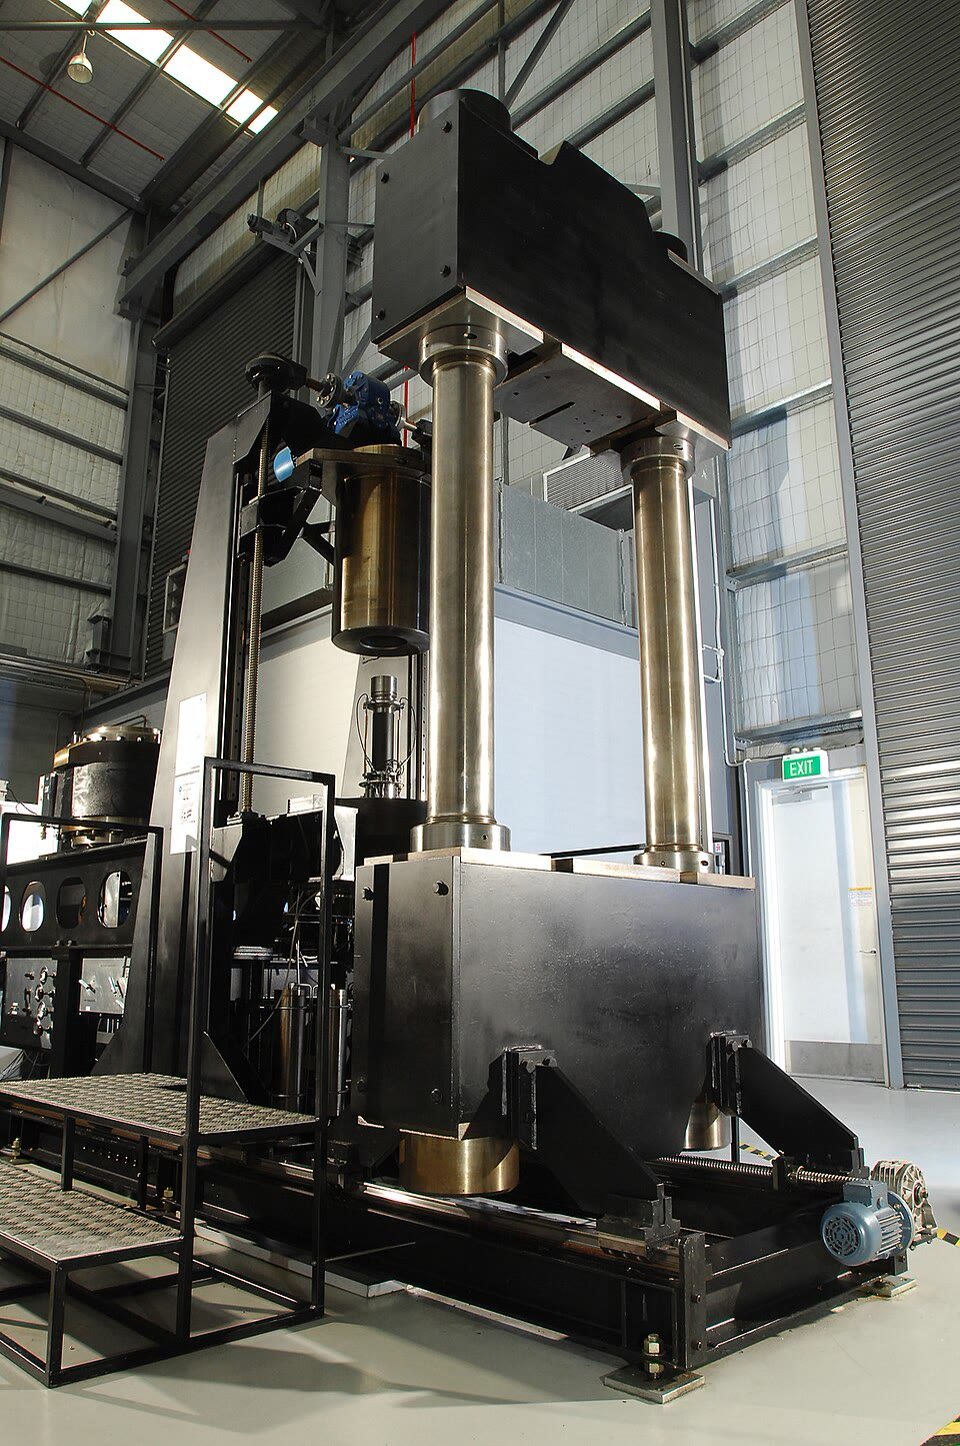
\includegraphics[width=\linewidth]{images/book3/b1-triaxial-cell.jpg}

{\scriptsize Sel triaksial tekanan tinggi untuk mengukur kekuatan batuan
(Darryl Peroni, CSIRO, CC BY 3.0).}
% ledger: commons:csiro-triaxial
\end{minipage}
\end{inthelab}

\section{Kekuatan litosfer}\label{sec:b1:stress-strain-rheology:envelope}

Pada setiap kedalaman \omterm{def:b1:layered-earth:lithosphere}{litosfer} dapat gagal dengan dua cara: dengan tergelincir pada sesar, dengan kekuatan yang tumbuh bersama tekanan efektif, atau dengan rayapan, dengan kekuatan yang turun ketika ia makin panas. Ia terdeformasi dengan cara mana pun yang memerlukan tegangan lebih kecil.

\begin{definition}[Amplop kekuatan, transisi rapuh--duktil, lapisan seismogenik]\label{def:b1:stress-strain-rheology:strength-envelope}
\emph{Amplop kekuatan}\index{amplop kekuatan} \omterm{def:b1:layered-earth:lithosphere}{litosfer} adalah kurva, terhadap kedalaman, dari \omterm{def:b1:stress-strain-rheology:principal}{tegangan diferensial} terbesar yang dapat ditahannya pada laju regangan tertentu: pada setiap kedalaman, yang lebih kecil dari kekuatan gesek dan kekuatan rayapan. \emph{Transisi rapuh--duktil}\index{transisi rapuh--duktil} adalah kedalaman tempat keduanya sama: di atasnya batuan terdeformasi dengan patahan, di bawahnya dengan rayapan. \emph{Lapisan seismogenik}\index{lapisan seismogenik} adalah rentang kedalaman tempat sebagian besar gempa bumi dimulai.
\end{definition}

\begin{proposition}[Kekuatan gesek terhadap kedalaman]\label{prop:b1:stress-strain-rheology:brittle-gradient}
Dalam lapisan dengan massa jenis $\rho$, dengan tekanan pori hidrostatik, satu \omterm{def:b1:stress-strain-rheology:principal}{tegangan utama} vertikal, sesar dari setiap orientasi dan tanpa \omterm{def:b1:stress-strain-rheology:coulomb}{kohesi}, tergelincir dengan gesekan $\mu$ dimulai pada \omterm{def:b1:stress-strain-rheology:principal}{tegangan diferensial}
\begin{align*}
  \sigma_1 - \sigma_3 &= \frac{2\mu}{\sqrt{1+\mu^2} + \mu}\,\rho g z(1-\lambda)
  && \text{jika $\sigma_v = \sigma_1$}, \\
  \sigma_1 - \sigma_3 &= \frac{2\mu}{\sqrt{1+\mu^2} - \mu}\,\rho g z(1-\lambda)
  && \text{jika $\sigma_v = \sigma_3$},
\end{align*}
dengan $\lambda = \rho_w/\rho$: kasus pertama memberi sesar normal, yang kedua sesar dorong.
\end{proposition}

\begin{proof}
\omterm{def:b1:stress-strain-rheology:lithostatic}{Tegangan efektif} vertikal adalah $S = \rho g z - \rho_w g z = \rho g z(1-\lambda)$.
Dengan $C = 0$ dan $k = \sqrt{1+\mu^2}$, \cref{thm:b1:stress-strain-rheology:failure-angle} mengatakan bahwa sesar tergelincir ketika $r = \mu c'/k$, dengan $r$ jari-jari dan $c'$ pusat lingkaran Mohr efektif. Jika $\sigma_v = \sigma_1$, maka
$\sigma_1' = S$ dan $c' = S - r$, sehingga $rk = \mu S - \mu r$ dan $r = \mu S/(k+\mu)$. Jika $\sigma_v = \sigma_3$, maka $c' = S + r$ dan $r = \mu S/(k-\mu)$. \omterm{def:b1:stress-strain-rheology:principal}{Tegangan diferensial} adalah $2r$.
\end{proof}

Dengan $\mu = 0.85$ dan $\rho = \qty{2700}{kg.m^{-3}}$, $S$ bertambah sebesar \qty{16.7}{MPa} per kilometer dan kekuatan gesek sebesar \qty{13.1}{MPa} per kilometer di bawah \omterm{def:b1:stress-strain-rheology:strain}{peregangan} dan \qty{61.3}{MPa} per kilometer di bawah kompresi, hampir lima kali lebih banyak: \omterm{def:b1:layered-earth:layers}{kerak} jauh lebih mudah ditarik terpisah daripada didorong bersama. Melampaui \omterm{def:b1:stress-strain-rheology:stress}{tegangan normal} efektif \qty{200}{MPa}, cabang atas \omterm{prop:b1:stress-strain-rheology:byerlee}{hukum Byerlee} mengambil alih, dan \omterm{def:b1:geological-maps:attitude}{kemiringannya} turun, dalam kompresi, menjadi sekitar \qty{35}{MPa} per kilometer.
% computed in figdata/bachelor-1/strength_envelope.py (tested); ledger: byerlee:1975

\begin{omfigure}
\begin{tikzpicture}
\pgfplotsset{envaxis/.style={omrecord, omdepth, scale only axis, width=5.6cm, height=7.2cm,
  xmin=-1000, xmax=2500, ymin=0, ymax=80, xtick={-1000,0,1000,2000},
  ytick={0,10,...,80}, unbounded coords=jump,
  xlabel={tegangan diferensial $\sigma_1-\sigma_3$ (MPa)},
  tick label style={font=\scriptsize}, label style={font=\small},
  scaled x ticks=false, xticklabel style={/pgf/number format/.cd, 1000 sep={\,}}}}
% computed in figdata/bachelor-1/strength_envelope.py; ledger: byerlee:1975, lopez:flow-laws, codata:R, prem:moho-average
\begin{axis}[envaxis, name=cont, ylabel={kedalaman (km)}, title={\small (a) benua, \qty{55}{mW.m^{-2}}}]
\addplot[fill=omLithGranite!45, draw=none] table[x=x, y=depth] {figdata/out/bachelor-1-strength_envelope-continental-outline.dat};
\addplot[omThm, line width=0.5pt, restrict x to domain=-1:2450] table[x=thrust, y=depth] {figdata/out/bachelor-1-strength_envelope-continental.dat};
\addplot[omThm, line width=0.5pt, restrict x to domain=-2450:1] table[x expr=-\thisrow{normal}, y=depth] {figdata/out/bachelor-1-strength_envelope-continental.dat};
\addplot[omDef, line width=0.5pt, restrict x to domain=-1:2450] table[x=ductile, y=depth] {figdata/out/bachelor-1-strength_envelope-continental.dat};
\addplot[omDef, line width=0.5pt, restrict x to domain=-2450:1] table[x expr=-\thisrow{ductile}, y=depth] {figdata/out/bachelor-1-strength_envelope-continental.dat};
\addplot[black, line width=1.0pt] table[x=x, y=depth] {figdata/out/bachelor-1-strength_envelope-continental-outline.dat};
\draw[black!60, dashed] (axis cs:-1000,35) -- (axis cs:2500,35);
\node[font=\scriptsize, anchor=south east] at (axis cs:2480,35) {Moho};
\draw[black, densely dotted] (axis cs:0,0) -- (axis cs:0,80);
\draw[black!70] (axis cs:660,13.7) -- (axis cs:1700,18) node[anchor=north, font=\scriptsize, align=center, text=black] {transisi\\ \qty{14}{km}};
\draw[black!70] (axis cs:1870,44.6) -- (axis cs:1950,53) node[anchor=north, font=\scriptsize, align=center, text=black] {transisi\\ mantel};
\node[font=\scriptsize, anchor=north, omThm] at (axis cs:1500,3) {kompresi};
\node[font=\scriptsize, anchor=north, omThm] at (axis cs:-560,3) {peregangan};
\node[font=\scriptsize, anchor=west, omDef] at (axis cs:40,31) {kuarsa basah};
\node[font=\scriptsize, anchor=west, omDef] at (axis cs:300,66) {olivin kering};
\end{axis}
\begin{axis}[envaxis, at={(cont.east)}, anchor=west, xshift=0.6cm, yticklabels={}, title={\small (b) dasar samudra berumur \qty{60}{Ma}}]
\addplot[fill=omLithBasalt!45, draw=none] table[x=x, y=depth] {figdata/out/bachelor-1-strength_envelope-oceanic-outline.dat};
\addplot[omThm, line width=0.5pt, restrict x to domain=-1:2450] table[x=thrust, y=depth] {figdata/out/bachelor-1-strength_envelope-oceanic.dat};
\addplot[omThm, line width=0.5pt, restrict x to domain=-2450:1] table[x expr=-\thisrow{normal}, y=depth] {figdata/out/bachelor-1-strength_envelope-oceanic.dat};
\addplot[omDef, line width=0.5pt, restrict x to domain=-1:2450] table[x=ductile, y=depth] {figdata/out/bachelor-1-strength_envelope-oceanic.dat};
\addplot[omDef, line width=0.5pt, restrict x to domain=-2450:1] table[x expr=-\thisrow{ductile}, y=depth] {figdata/out/bachelor-1-strength_envelope-oceanic.dat};
\addplot[black, line width=1.0pt] table[x=x, y=depth] {figdata/out/bachelor-1-strength_envelope-oceanic-outline.dat};
\draw[black, densely dotted] (axis cs:0,0) -- (axis cs:0,80);
\draw[black!70] (axis cs:2003,38.2) -- (axis cs:1900,50) node[anchor=north, font=\scriptsize, align=center, text=black] {transisi\\ \qty{38}{km}};
\node[font=\scriptsize, anchor=west, omDef] at (axis cs:300,66) {olivin kering};
\end{axis}
\end{tikzpicture}
\par\smallskip{\small \omterm{def:b1:stress-strain-rheology:strength-envelope}{Amplop kekuatan} pada laju regangan \qty{e-15}{s^{-1}}. Merah: kekuatan gesek dari \omterm{prop:b1:stress-strain-rheology:byerlee}{hukum Byerlee} dengan tekanan pori hidrostatik, untuk kompresi (sesar dorong, kanan) dan \omterm{def:b1:stress-strain-rheology:strain}{peregangan} (sesar normal, kiri, digambar negatif); biru: kekuatan rayapan kuarsit basah di \omterm{def:b1:layered-earth:layers}{kerak} benua dan \omterm{def:b1:rock-forming-minerals:groups}{olivin} kering di \omterm{def:b1:layered-earth:layers}{mantel}; garis tepi hitam dan arsiran: kekuatannya, yang lebih kecil dari keduanya pada setiap kedalaman. (a) Benua dengan \omterm{def:b1:heat-budget:heat-flow}{aliran panas} permukaan \qty{55}{mW.m^{-2}} dan \omterm{def:b1:layered-earth:layers}{kerak} setebal \qty{35}{km}: \omterm{def:b1:layered-earth:layers}{kerak} atas yang kuat, \omterm{def:b1:layered-earth:layers}{kerak} bawah yang lemah, \omterm{def:b1:layered-earth:layers}{mantel} paling atas yang kuat. (b) Dasar samudra berumur \qty{60}{Ma}: satu lapisan kuat, setebal \qty{38}{km} dalam kompresi.}
\label{fig:b1:stress-strain-rheology:envelope}
\end{omfigure}

Gambar di atas menggabungkan kedua kekuatan untuk dua \omterm{def:b1:layered-earth:lithosphere}{litosfer}. Benua memiliki \omterm{def:b1:heat-budget:geotherm}{geoterm} \cref{ch:b1:heat-budget} dengan \omterm{def:b1:heat-budget:heat-flow}{aliran panas} permukaan \qty{55}{mW.m^{-2}}, \omterm{def:b1:layered-earth:layers}{kerak} kuarsit basah setebal \qty{35}{km}, dan \omterm{def:b1:rock-forming-minerals:groups}{olivin} kering di bawahnya; dasar samudra berumur \qty{60}{Ma}, dengan \omterm{def:b1:heat-budget:geotherm}{geoterm} setengah-ruang dari bab yang sama, dan \omterm{def:b1:rock-forming-minerals:groups}{olivin} dari dasar laut ke bawah. Laju regangannya \qty{e-15}{s^{-1}}. \qty{35}{km} adalah kedalaman rata-rata \omterm{def:b1:layered-earth:discontinuity}{Moho} di bawah benua dalam \omterm{def:b1:layered-earth:reference-model}{model acuan Bumi} \cref{ch:b1:layered-earth}.
% ledger: prem:moho-average

Di bawah benua \omterm{def:b1:stress-strain-rheology:strength-envelope}{transisi rapuh--duktil} jatuh pada \qty{13.7}{km} dalam kompresi, pada \qty{249}{\degreeCelsius}, dan pada \qty{17.1}{km} dalam \omterm{def:b1:stress-strain-rheology:strain}{peregangan}. \omterm{def:b1:layered-earth:layers}{Kerak} yang lebih hangat akan menaikkannya, dan yang lebih dingin menurunkannya, karena hukum rayapan bergantung pada suhu saja pada tegangan tertentu. Transisi itu adalah tingkat terkuat \omterm{def:b1:layered-earth:layers}{kerak}.
Di bawahnya kekuatan runtuh: di \omterm{def:b1:layered-earth:discontinuity}{Moho}, pada \qty{527}{\degreeCelsius}, kuarsit mengalir di bawah \qty{7.6}{MPa}, sedangkan \omterm{def:b1:rock-forming-minerals:groups}{olivin} pada suhu yang sama memerlukan sekitar \qty{30000}{MPa}, jauh melampaui kekuatan gesek sehingga bagian atas \omterm{def:b1:layered-earth:layers}{mantel} kembali rapuh. Transisi kedua mengikuti pada \qty{44.6}{km} dalam kompresi. \omterm{def:b1:layered-earth:layers}{Kerak} bawah model ini adalah lapisan lunak di antara dua lapisan kuat: ``sandwich jeli''. Di bawah samudra seluruh \omterm{def:b1:layered-earth:lithosphere}{litosfer} adalah \omterm{def:b1:rock-forming-minerals:groups}{olivin}, dan kekuatannya tumbuh ke bawah hingga satu transisi tunggal pada \qty{38.2}{km}, pada \qty{641}{\degreeCelsius}.
% computed in figdata/bachelor-1/strength_envelope.py (tested)

Gempa bumi sesuai dengan amplop samudra: di dalam lempeng samudra, mereka mencapai kedalaman tempat suhunya \qtyrange{600}{800}{\degreeCelsius}, dekat dengan \qty{641}{\degreeCelsius} transisi tunggal model itu. Gempa yang lebih dalam hanya terjadi di tempat satu lempeng menunjam di bawah yang lain, hingga lebih dari \qty{700}{km} (\cref{ch:b1:active-margins}).
% ledger: jackson:jelly, usgs:deepest

\omterm{def:b1:layered-earth:layers}{Mantel} benua adalah tempat gambarannya diperdebatkan. Selama sekitar dua puluh tahun sandwich jeli adalah pandangan yang berlaku, dibangun di atas pengukuran laboratorium \omterm{def:b1:rock-forming-minerals:groups}{olivin} kering dan atas beberapa gempa bumi yang diduga berada di bawah \omterm{def:b1:layered-earth:discontinuity}{Moho}. Pada 2002 James Jackson berpendapat bahwa ia harus ditinggalkan: kedalaman yang lebih baik menunjukkan bahwa gempa bumi di benua terbatas pada satu lapisan, biasanya \omterm{def:b1:layered-earth:layers}{kerak} atas, kadang seluruh \omterm{def:b1:layered-earth:layers}{kerak}, tanpa gempa bumi yang meyakinkan di \omterm{def:b1:layered-earth:layers}{mantel} di bawahnya, bahkan di tempat \omterm{def:b1:layered-earth:discontinuity}{Moho} hanya \qtyrange{300}{500}{\degreeCelsius}. Sedikit air, beberapa bagian per juta dalam \omterm{def:b1:rock-forming-minerals:groups}{olivin}, cukup untuk melemahkannya secara drastis, dan \omterm{def:b1:layered-earth:layers}{mantel} benua mungkin memang memuat sebanyak itu; kekuatan benua kemudian sebagian besar terletak di \omterm{def:b1:layered-earth:layers}{kerak} mereka. Kedua pandangan menggambar amplop yang berbeda dari hukum yang sama, dengan \omterm{def:b1:rock-forming-minerals:groups}{olivin} kering atau basah di bawah \omterm{def:b1:layered-earth:discontinuity}{Moho}.
% ledger: jackson:jelly
Apa pun yang benar, amplop adalah batas dan bukan pengukuran: hukum laboratorium diekstrapolasi melalui banyak orde besaran laju regangan, dan tegangan puncak yang ditunjukkannya, lebih dari satu gigapascal, jauh di atas \qtyrange{1}{10}{MPa} yang terlihat dilepaskan gempa bumi.
% ledger: jackson:jelly

\section{Latihan}

\begin{exercise}[$\star$]\label{exo:b1:stress-strain-rheology:1}
Ambil \omterm{def:b1:layered-earth:layers}{kerak} dengan massa jenis \qty{2700}{kg.m^{-3}} dan $g = \qty{9.81}{m.s^{-2}}$. Pada kedalaman \qty{10}{km}, hitung (a) tegangan vertikal, (b) tekanan pori hidrostatik, (c) \omterm{def:b1:stress-strain-rheology:lithostatic}{tegangan efektif} vertikal dan rasio tekanan pori $\lambda$.
\end{exercise}

\begin{exercise}[$\star$]\label{exo:b1:stress-strain-rheology:2}
(a) Sebuah lapisan sepanjang \qty{10}{km} diregangkan hingga \qty{13}{km}: berikan \omterm{def:b1:stress-strain-rheology:strain}{perpanjangan} dan perengangannya. (b) Lapisan lain, sepanjang \qty{10}{km}, dipendekkan hingga \qty{7}{km}. (c) Dua garis batuan yang tadinya tegak lurus kini membentuk sudut \ang{60}: berapa sudut geser dan \omterm{def:b1:stress-strain-rheology:strain}{regangan gesernya}?
\end{exercise}

\begin{exercise}[$\star$]\label{exo:b1:stress-strain-rheology:3}
Pada suatu titik, $\sigma_1 = \qty{100}{MPa}$ dan $\sigma_3 = \qty{40}{MPa}$. (a) Gambarkan lingkaran Mohr. (b) Berapa tegangan geser terbesar, pada bidang mana ia bekerja, dan \omterm{def:b1:stress-strain-rheology:stress}{tegangan normal} apa yang bekerja pada bidang-bidang itu? (c) Hitung $\sigma_n$ dan $\tau$ pada bidang yang normalnya membentuk \ang{30} dengan $\sigma_1$.
\end{exercise}

\begin{exercise}[$\star$]\label{exo:b1:stress-strain-rheology:4}
Sebuah batuan memiliki \omterm{def:b1:stress-strain-rheology:coulomb}{kohesi} \qty{10}{MPa} dan \omterm{def:b1:stress-strain-rheology:coulomb}{sudut gesekan internal} \ang{30}. (a) Pada sudut berapa terhadap $\sigma_1$ ia pecah, dan sudut apa yang dibentuk oleh kedua bidang rekahan yang mungkin satu sama lain? (b) Dengan $\sigma_3' = \qty{20}{MPa}$, $\sigma_1'$ efektif berapa yang memecahkannya?
\end{exercise}

\begin{exercise}[$\star\star$]\label{exo:b1:stress-strain-rheology:5}
Dalam sumbu $x$ (horizontal) dan $y$ (vertikal), $\sigma_{xx} = \qty{60}{MPa}$, $\sigma_{yy} = \qty{20}{MPa}$ dan $\sigma_{xy} = \qty{15}{MPa}$. (a) Hitung \omterm{def:b1:stress-strain-rheology:principal}{tegangan utama} dan sudut $\theta_p$. (b) Periksa dengan \cref{prop:b1:stress-strain-rheology:transformation} bahwa bidang dengan normal $\theta_p$ tidak membawa tegangan geser dan \omterm{def:b1:stress-strain-rheology:stress}{tegangan normal} $\sigma_1$. (c) Berapa tegangan geser terbesar pada titik ini?
\end{exercise}

\begin{exercise}[$\star\star$]\label{exo:b1:stress-strain-rheology:6}
Sebuah zona geser telah mendeformasi batuannya dengan \omterm{def:b1:stress-strain-rheology:shear-types}{geser sederhana} $\gamma = 2$. (a) Hitung \omterm{def:b1:stress-strain-rheology:strain}{peregangan} utama dan sudut sumbu panjang \omterm{def:b1:stress-strain-rheology:strain-ellipse}{elips regangan} terhadap arah geser. (b) Periksa bahwa luasnya tidak berubah. (c) Sebuah garis bahan berada pada \ang{45} terhadap arah geser, naik searah dengan geser: di mana ia sekarang, dan berapa \omterm{def:b1:stress-strain-rheology:strain}{peregangannya}? Bandingkan dengan (a).
\end{exercise}

\begin{exercise}[$\star\star$]\label{exo:b1:stress-strain-rheology:7}
Dalam zona geser setebal \qty{200}{m}, bintik-bintik bulat kecil dalam batusabak telah menjadi elips dengan sumbu dalam perbandingan 4 banding 1. Anggap \omterm{def:b1:stress-strain-rheology:shear-types}{geser sederhana}, tanpa perubahan luas. (a) Cari $S_1$, $S_2$ dan $\gamma$. (b) Pada sudut berapa terhadap dinding zona itu sumbu panjangnya harus terletak? (c) Seberapa jauh satu dinding telah bergerak melewati yang lain?
\end{exercise}

\begin{exercise}[$\star\star$]\label{exo:b1:stress-strain-rheology:8}
Sebuah sesar pada kedalaman \qty{3}{km}, dalam \omterm{def:b1:layered-earth:layers}{kerak} dengan massa jenis \qty{2700}{kg.m^{-3}}, memikul \omterm{def:b1:stress-strain-rheology:stress}{tegangan normal} \qty{70}{MPa} dan tegangan geser \qty{30}{MPa}. (a) Dengan tekanan pori hidrostatik, apakah ia tergelincir menurut \omterm{prop:b1:stress-strain-rheology:byerlee}{hukum Byerlee}? (b) Bagaimana jika porinya tersegel dan $\lambda = 0.6$? (c) Cari nilai $\lambda$ pada saat ia mulai tergelincir.
\end{exercise}

\begin{exercise}[$\star\star$]\label{exo:b1:stress-strain-rheology:9}
Gunakan hukum rayapan kuarsit basah (\cref{prop:b1:stress-strain-rheology:creep}). (a) Dengan faktor berapa tegangan harus naik agar ia mengalir sepuluh kali lebih cepat? (b) Dengan faktor berapa kekuatannya turun antara \qty{400}{\degreeCelsius} dan \qty{500}{\degreeCelsius}, pada laju yang sama dan dengan $V = 0$? (c) Jelaskan dengan kedua hasil ini mengapa kedalaman \omterm{def:b1:stress-strain-rheology:strength-envelope}{transisi rapuh--duktil} jauh lebih bergantung pada \omterm{def:b1:heat-budget:geotherm}{geoterm} daripada pada laju regangan.
\end{exercise}

\begin{exercise}[$\star\star\star$]\label{exo:b1:stress-strain-rheology:10}
Di mana tegangan vertikal adalah $\sigma_2$, sesar adalah sesar geser-mendatar. Anggap bahwa \omterm{def:b1:stress-strain-rheology:lithostatic}{tegangan efektif} vertikal kemudian adalah rata-rata $(\sigma_1' + \sigma_3')/2$. (a) Tunjukkan bahwa tergelincir dengan gesekan $\mu$ dan tanpa \omterm{def:b1:stress-strain-rheology:coulomb}{kohesi} dimulai pada $\sigma_1 - \sigma_3 = 2\mu\,\rho g z(1-\lambda)/\sqrt{1+\mu^2}$. (b) Hitung gradiennya dalam megapascal per kilometer untuk $\mu = 0.85$ dan $\rho = \qty{2700}{kg.m^{-3}}$, dan letakkan di antara gradien sesar normal dan sesar dorong. (c) Nyatakan masing-masing dari ketiga gradien sebagai kelipatan tegangan vertikal efektif.
\end{exercise}

\begin{exercise}[$\star\star\star$]\label{exo:b1:stress-strain-rheology:11}
Modelkan \omterm{def:b1:layered-earth:lithosphere}{litosfer} samudra berumur \qty{60}{Ma} sebagai setengah-ruang yang didinginkan dari \qty{1350}{\degreeCelsius}, dengan permukaan pada \qty{0}{\degreeCelsius} dan $\kappa = \qty{e-6}{m^2.s^{-1}}$: $T = \num{1350}\operatorname{erf}\bigl(z/(2\sqrt{\kappa t})\bigr)$. (a) Hitung $2\sqrt{\kappa t}$. (b) Cari kedalaman isoterm \qty{600}{\degreeCelsius} dan \qty{800}{\degreeCelsius}. (c) Gempa bumi di dalam lempeng samudra mencapai kedalaman tempat suhunya \qtyrange{600}{800}{\degreeCelsius}. Bandingkan dengan \omterm{def:b1:stress-strain-rheology:strength-envelope}{transisi rapuh--duktil} dalam \omterm{def:b1:stress-strain-rheology:strength-envelope}{amplop kekuatan} samudra bab ini, pada \qty{38.2}{km} dan \qty{641}{\degreeCelsius}.
% ledger: jackson:jelly
\end{exercise}

\begin{exercise}[$\star\star\star$]\label{exo:b1:stress-strain-rheology:12}
Sebuah batuan dilintasi rekahan dari setiap orientasi, semuanya memuat arah $\sigma_2$, tanpa \omterm{def:b1:stress-strain-rheology:coulomb}{kohesi} dan gesekan 0.85. \omterm{def:b1:stress-strain-rheology:principal}{Tegangan utama} efektifnya adalah $\sigma_1' = \qty{110}{MPa}$ dan $\sigma_3' = \qty{20}{MPa}$. (a) Tunjukkan bahwa beberapa rekahan tergelincir. (b) Cari rentang sudut antara rekahan yang tergelincir dan $\sigma_1$. Yang manakah yang berada di tengah rentang itu? (c) Sampai nilai $\sigma_1'$ berapa, dengan $\sigma_3'$ tetap, setidaknya satu rekahan masih tergelincir?
\end{exercise}

\section{Masalah: Akankah sesar tergelincir?}

\begin{problem}[{Soal akhir pekan --- tegangan pada sesar normal pada kedalaman lima kilometer, margin keamanannya, dan kenaikan tekanan pori yang akan membuatnya tergelincir}]
\label{pb:b1:stress-strain-rheology:1}
% values: calc/ch16.py; ledger: byerlee:1975, hb81:denver
Sebuah sesar berjurus utara--selatan dan miring \ang{60} ke timur. Sebuah sumur pembuangan mencapainya pada kedalaman \qty{5.00}{km}, dalam \omterm{def:b1:layered-earth:layers}{kerak} dengan massa jenis \qty{2700}{kg.m^{-3}} yang porinya terhubung ke permukaan. Sebuah pengukuran di dalam sumur memberi tegangan horizontal tegak lurus sesar, \qty{75.0}{MPa}; tegangan horizontal sepanjang \omterm{def:b1:geological-maps:attitude}{jurus} berada di antara itu dan tegangan vertikal, sehingga soalnya dua dimensi dalam bidang vertikal timur--barat. Ambil $g = \qty{9.81}{m.s^{-2}}$, air dengan massa jenis \qty{1000}{kg.m^{-3}} dan \omterm{prop:b1:stress-strain-rheology:byerlee}{hukum Byerlee}. Berikan tegangan hingga \qty{0.01}{MPa}.

\medskip
\noindent\textbf{Bagian I --- Keadaan tegangan.}
\begin{enumerate}
  \item Hitung tegangan vertikal pada kedalaman sesar.
  \item Hitung tekanan pori hidrostatik di sana, dan rasio $\lambda$.
  \item Manakah dari kedua tegangan itu yang $\sigma_1$ dan yang $\sigma_3$? Jenis sesar apa yang didorong oleh keadaan tegangan ini?
  \item Hitung \omterm{def:b1:stress-strain-rheology:principal}{tegangan diferensial}, pusat dan jari-jari lingkaran Mohr.
  \item Hitung \omterm{def:b1:stress-strain-rheology:principal}{tegangan utama} efektif dan pusat lingkaran efektif.
  \item Dengan $x$ horizontal ke timur dan $y$ vertikal, tuliskan ketiga komponen $\sigma_{xx}$, $\sigma_{yy}$, $\sigma_{xy}$. Mengapa $\sigma_{xy}$ nol?
\end{enumerate}

\medskip
\noindent\textbf{Bagian II --- Tegangan pada sesar.}
\begin{enumerate}[resume]
  \item Berikan normal satuan sesar dalam sumbu pada soal 6, dan sudut $\theta$ antara normal itu dan $\sigma_1$.
  \item Hitung $\sigma_n$ dan $\tau$ pada sesar dengan \cref{prop:b1:stress-strain-rheology:transformation}.
  \item Periksa kedua nilai dengan lingkaran Mohr: pada sudut berapa dari ujung $\sigma_1$ sesar itu terletak?
  \item Hitung \omterm{def:b1:stress-strain-rheology:stress}{tegangan normal} efektif pada sesar.
  \item Hitung rasio $\tau/\sigma_n'$ dan bandingkan dengan 0.85.
  \item Tegangan geser berapa yang akan membuat sesar tergelincir di bawah \omterm{def:b1:stress-strain-rheology:stress}{tegangan normal} efektif sekarang? Dengan berapa megapascal ia kurang?
\end{enumerate}

\medskip
\noindent\textbf{Bagian III --- Lingkaran Mohr dan hukum Byerlee.}
\begin{enumerate}[resume]
  \item Gambarkan lingkaran Mohr efektif dan garis Byerlee dengan skala.
  \item Hitung jarak dari pusat lingkaran ke garis dan bandingkan dengan jari-jarinya. Dapatkah bidang mana pun melalui batuan itu tergelincir?
  \item Bidang manakah yang akan tergelincir lebih dulu? Berikan sudutnya terhadap $\sigma_1$ dan \omterm{def:b1:geological-maps:attitude}{kemiringannya}.
  \item Dengan \cref{prop:b1:stress-strain-rheology:brittle-gradient}, hitung \omterm{def:b1:stress-strain-rheology:principal}{tegangan diferensial} pada saat sesar normal tergelincir pada kedalaman ini, dan periksa dengan gradien \qty{13.1}{MPa} per kilometer.
  \item Seberapa rendah tegangan horizontal harus turun agar bidang yang paling baik orientasinya tergelincir?
  \item Seberapa rendah untuk sesar dalam soal ini agar tergelincir? Jelaskan mengapa ia lebih rendah.
\end{enumerate}

\medskip
\noindent\textbf{Bagian IV --- Injeksi.}
\begin{enumerate}[resume]
  \item Jelaskan mengapa kenaikan $\Delta P$ pada tekanan pori menggeser lingkaran efektif sejauh $\Delta P$ ke kiri tanpa mengubah jari-jarinya.
  \item Hitung kenaikan tekanan pori yang membuat bidang yang paling baik orientasinya tergelincir.
  \item Sumur penuh dengan air. Tekanan ekstra apa yang harus diberikan pompa di kepala sumur untuk menaikkan tekanan pori di sesar sebesar jumlah itu? Setinggi apa kolom air yang setara dengannya?
  \item Jika gesekan pada sesar 0.6 alih-alih 0.85, apakah ia sudah tergelincir? Apa yang dikatakan ketenangan sesar tentang gesekannya?
  \item Pada rasio $\lambda$ berapa bidang yang paling baik orientasinya tergelincir?
  \item Hingga satu desimal, dalam megapascal, kenaikan tekanan pori berapa yang membuat sesar ini tergelincir?
\end{enumerate}
\end{problem}
